\documentclass[../main]{subfiles}
\begin{document}

\chapter{Private key authentication schemes}

\section{Difference between secrecy and authentication}

\begin{figure}[h]
    \centering
    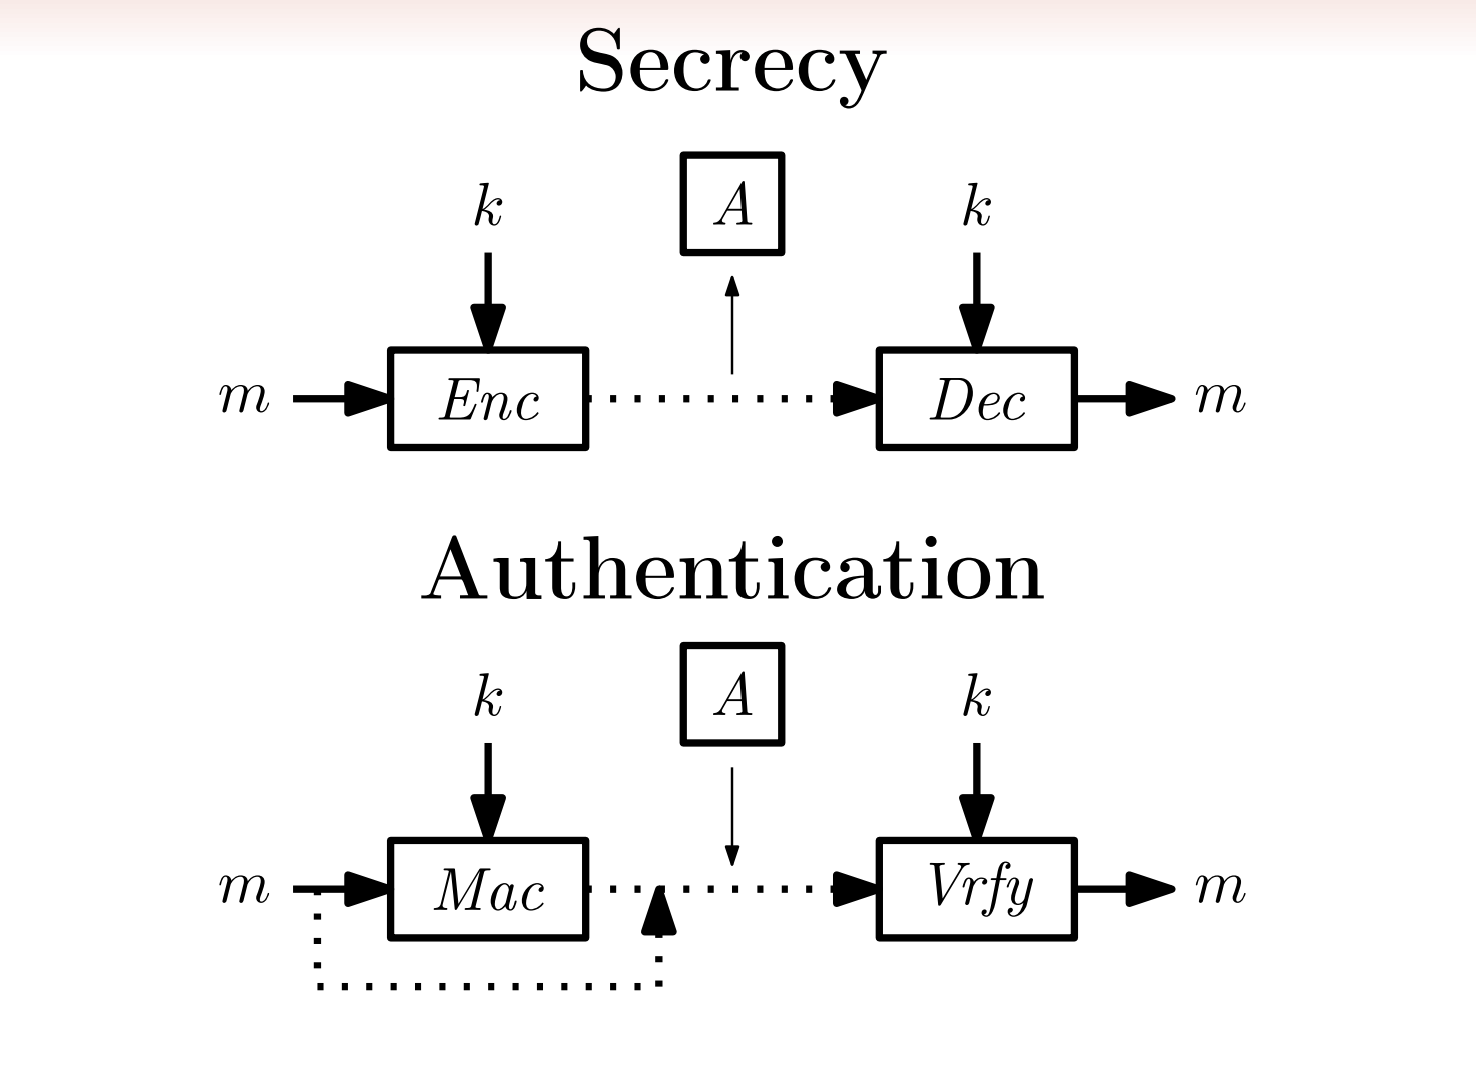
\includegraphics[width=0.5\textwidth]{images/difference_secrecy_authentication}
    \caption{Difference between secrecy and authentication.}
\end{figure}

In secrecy schemes, the channel is secure and the focus of the adversary is reading what goes through the channel. 
In authentication schemes, the channel is not secure and the focus of the adversary is not to read the content of the channel, but to write on it.
That is why the receiver wants to be sure that the message sent along the channel is actually coming from the expected sender.
For that we need a \textbf{Message Authentication Code (MAC)}.\\
\noindent
Authentication and secrecy are different: solving the problem of secrecy does not solve the problem of authentication.
We do not want adversaries to be able to \textit{forge} messages of their choice $m$ without knowing a key $k$.

\section{Message Authentication Codes}
The same way ciphers guarantee secrecy, \textbf{Message Authentication Codes (MACs)} guarantee authentication.
\begin{definition}
    A MAC is a triple $\Pi = (Gen, Mac, Vrfy)$ of PPT algorithms such that:
    \begin{itemize}
        \item $Gen$ takes as input a string in the form $1^n$ (the security parameter) and outputs a key $k$ which can be such that $|k|\ge n$.
        \item $Mac$ takes as input a key $k$ and a message $m$ and outputs a \textbf{tag} $t$.
        \item $Vrfy$ takes as input a key $k$, a message $m$ and a tag $t$, and outputs a boolean $b$.
    \end{itemize}
    A MAC $\Pi = (Gen, Mac, Vrfy)$ is \textit{correct} when $Vrfy(k, m, Mac(k, m)) = true$.
\end{definition}

\noindent
In order to be safe and sound, the assumptions are very pessimistic:
\begin{itemize}
    \item the adversary $A$ has access to an oracle $Mac_k(\cdot)$ which can be used to generate all possible tags;
    \item having access to a previously generated pair ($m$,$t$) is not interesting;
    \item $A$ has to be PPT;
    \item the new experiment is called $MacForge_{A,\Pi}(n)$.
\end{itemize}

\noindent
Let us present the new experiment:\\
$MacForge_{A,\Pi}(n):$\\
$k \leftarrow{} Gen(1^n)$\\
$(m,t) \leftarrow{} A(1^n,Mac_k(\cdot))$\\
$\mathbb{Q} \leftarrow{} \{m \; | \; A$ queries $Mac_k(\cdot)$ on $m\}$\\
\textbf{Result:} ($m \notin{\mathbb{Q}} \wedge{} Vrfy(k,m,t) = true$)

\begin{definition}
    A MAC $\Pi$ is secure if and only if for every adversary PPT $A$ there exists a function $\varepsilon{} \in{} \mathcal{NGL}$ such that:
    $$Pr(MacForge_{\Pi,A}(n) = 1) = \varepsilon(n)$$
\end{definition}
\end{document}